\chapter{Protocol Translation}
\label{sec:imperative_form}

The task of the Reo compiler is to translate a Reo protocol specification into the target language. The resulting code must interface with other components written in the language such that, at runtime, the resulting system behaves as specified. In this chapter, we explain how we extend the Reo compiler to support the Rust language target.

Section~\ref{sec:two_phase} examines the task of the backend, breaking it down into smaller, more specialized subtasks. Section~\ref{sec:decoupling_reo_rust} organizes these subtasks into a pipeline that sees the translation through from Reo specification to executable Rust protocol object. By design, this process transforms the protocol from one form to another. To bridge the gap between Reo and Rust compilers, Section~\ref{sec:imperative_form} defines \textit{imperative form} as a new representation of a protocol's behavior in a manner conducive to imperative languages. Concretely, the Reo compiler emits Rust source code, whose contents are primarily a Rust-embedded representation of imperative form. Section~\ref{sec:translation_pipeline} goes into detail about the implementation of the translation pipeline by explaining how the previously-defined subtasks are completed in stages.

%\hl{
%	The task of the Reo compiler is to translate a Reo protocol specification into the target language. The resulting code must interface with other components written in the language such that, at runtime, the resulting system behaves as specified. Rust is an example of an imperative language, unable to represent port interactions at the same high level. Our generated code must implement the specification in terms of imperative actions
%	
%	Imperative languages must instead 
%	between a set of \textit{components} written in the target language. When connected together in the manner corresponding to the s
%	
%	the task is to generate a rust protocol object from the reo spec such that it can be used in a rust program.
%	3. naive extreme: 100 percent reo is infeasible: must do signficiant work emulating rust. and they both become tightly coupled
%	4. java solution is to move common object defs to a library. this is fine but its not enough! (WHY)
%	5. 
%	4. java recognized this problem and has the solution of using a lib for protocol and port. still, if we attempted to emulate this choice of granulairty, reo would still do the majority of the heavy lifting
%	5. we have a structured approach. isolate the tasks involved in the transformation. we identify that two are language-independent if beyond the target being imperative. 
%	6. we make this distinction concrete in considering it a two-step process with imperative form in the middle: representing the specification of an imperative protocol.
%	
%	3. follow the precedent of moving as much as possible to a library. minimizes repetition and avoids reo compiler from being too coupled on the implementation. on the other hand, moving things into the library prevent them from being entirely statically generated; forces us to express it in terms that can be computed at runtime. we strike a balance by performing all the high level transformations at runtime 
%}

%In this chapter, we describe the process of translating the Reo compiler's internal representation of a protocol specification into an executable \textit{protocol object} in the Rust language.

\section{Structuring the Translation Process}
\label{sec:two_phase}
In this section, we explore the nature of the task which characterizes the Rust backend for the Reo compiler. Section~\ref{sec:sub_tasks} breaks the problem down into simpler subtasks, and explains their relationship to one another and how they apply in the case of a different target language. Section~\ref{sec:decoupling_reo_rust} explains how these tasks are organized by defining their place within a translation pipeline. The implementation of the pipeline itself is given in Section~\ref{sec:translation_pipeline}.

\subsection{Translation Subtasks}
\label{sec:sub_tasks}
The Reo compiler's frontend parses its Reo input, and performs significant transformations on the resulting internal representation. Everything that follows is the task of the backend, transforming it further until code in the target language can be emitted. We define \textit{Reo Internal Representation} (RIR) to refer to the input of the backend in the sections to follow. Reo and Rust differ significantly in how they represent work. Accordingly, work expressed in the former must be transformed significantly before it can be expressed in the latter. In this section, this task is decomposed into \textit{subtasks}; their inclusion in the thesis serves a dual purpose: (1) smaller tasks are more easily understood, and help to characterize Reo and Rust by identifying their differences, and (2) only isolated subtasks can be separated, facilitating their organization into the translation pipeline shown in Section~\ref{sec:translation_pipeline}.

\subsubsection{Input Representation}
RIR embodies the completion of several of the operations on Reo connectors described in the literature~\cite{baier2006modeling, dokter2018rule}; namely, \textit{composition}, \textit{merging}, \textit{hiding}, and so on. For our purposes, it suffices to say that IR is presented in a form corresponding closely to an RBA, one of the semantic models described in Section~\ref{sec:semantic_models}. RIR is self-contained, and defines a list of \textit{rules} which correspond 1-to-1 to interactions between the protocol's ports. It captures the intuition of an RBA as they are usually understood in an imperative context; rules are subdivided into \textit{guard} and \textit{assignment}. Helpfully, IR presents the latter not as a monolithic formula, but rather as a mapping from identifier to \textit{term}. In our imperative context, terms can be understood as expressions whose evaluation at runtime will create new values.

\subsubsection{Conceptual Transformations}
Reo specifications represent connectors declaratively as relations between ports. They are thus well suited to reasoning about the protocol's properties. In contrast, our target imperative languages such as Java and Rust represent computation such that it corresponds more closely to machine instructions; they are imperative, laying out sequences of actions which together emerge as interaction at runtime. Where interactions in the former can be oriented around the synchronous observations of port values, interactions of the latter must be expressed as sequences of actions, laid out over time. IR is somewhere in between, per rule, the guard is distinguished from the assignment, distinguishing an ordering of operations at this binary granulaity: the guard is evaluated before values are assigned. This granularity requires further transformation before it can correspond with executable Rust. IR is able to disambiguate the order in which memory cells are read and written to by implying an ordering by annotating their identifiers with temporal \textit{qualifiers}. For example, the assignment corresponding to $m=A\wedge{}m'=B$ is declarative, but nevertheless suggests an ordering by annotating $m$ with a qualifier to represent its `future' value. Rust's imperative nature requires that operations on values occur in the order of their appearance in the programs control flow, such that they correspond with the order in which they are executed (Rust compiler optimizations notwithstanding).

Java, Rust and Reo have in common that they are strongly-typed languages. In the broader sense, `type' describes the classification of just about everything in Reo, including connectors and primitives. The Reo compiler's internals perform transformations that handle the majority of what could be considered `type checking'. The only exceptions are (1) the data types of each port, determining the types of values they transmit, and (2) the types of functions applied to values within the channel, which are  related to their identifiers by only an identifier. 
of \textit{type elision}; for the sake of programmer ergonomics, the data types of ports may be omitted, such that they can later be derived in context. Rust shares this property, and so the Rust compiler works to \textit{resolve} data types during compilation. Circumstantially, these elisions may produce cases for which a correct resolution is impossible, as the type annotations or constraints present are in conflict. Our task is to emulate this work ourselves, assigning concrete types for port objects in our emitted code such that is guaranteed to type check in the Rust language. Failure to do this correctly would result in Reo emitting code rejected by the Rust compiler. This would not be a threat to correctness, but it results in significant inconvenience to the programmer.

\subsubsection{From Specification to Implementation}
Regardless of any intermediate representation, protocols must ultimately be emitted in the target language at the required level of specificity. Imperative languages place the burden of defining \textit{how} their work is performed squarely on the shoulders on the programmer. We refer to this notion as the difference between specification and implementation.\footnote{These abstract concepts tend to fall apart under scrutiny, as they depend on what is meant by `computation' at all. Nevertheless, this observation is helpful in the context of our problem, as we prescribe the relationship between Reo and Rust by using the former to `model' the latter.} For example, where a declarative language might not distinguish \textit{merge sort} from \textit{bubble sort}, Rust certainly does; a Rust programmer operations on variables which correspond (relatively) closely to machine instructions as they will be executed at runtime. This is also true in the case of our problem; what is implied in Reo must be made explicit in Rust. This includes the initialization of system resources, operations on concurrency primitives, and all the minutia necessary to implement the optimizations described in Section~\ref{sec:behavior_implementation}. 

It is beneficial to recognize that a significant portion of the translation from Reo to Rust would be shared by the same procedure to a similar language; the more similar language, the more we can expect their respective transformations to have in common. For example, despite their significant differences, Rust and Java are more similar to each other than they are to Reo. Reo's role is to augment another language with coordination logic. Therefore, it seems to be a reasonable assumption that the majority of languages targeted by the Reo compiler would differ from Reo, such that they can benefit most from the abstractions Reo introduces. Imperative languages are a sensible choice, and so it is reasonable to assume that there is benefit in Reo supporting other imperative languages in future. To this end, we choose to distinguish translation subtasks according to whether they are relevant to Rust in particular, or are generally-applicable to an imperative target language.

It is beneficial to recognize that much of the work required for transforming Reo to Rust would be unchanged if another imperative language were selected as the target. For example, Java required that actions be laid out in accordance with the control flow of the program in the same manner as Rust. To capture this intuition, it helps to split our transformations into \textit{abstract} and \textit{concrete} phases, such that the former is not specific to the target imperative language. 

\subsubsection{Translation Subtasks Defined}

Ultimately, we partition the task of translating from IR to Rust as four subtasks, where those that are \textit{abstract} must precede those that are \textit{concrete}:

\begin{tabular}{l|p{5cm}p{5cm}}
	& Action & Data Type \\
	\hline
	Abstract & $T_{AA}$: From each abstract interaction, a sequence of abstract imperative actions are laid out. & $T_{AT}$: Ports are mapped to symbolic data types characterized by constraints on their properties. \\
	\hline
	Concrete & $T_{CA}$: Abstract actions are reified into concrete, executable Rust operations. & $T_{CT}$: Each symbolic data type is made concrete, selecting a particular Rust type.
\end{tabular}


%
%
%
%Aside from expression in the correct syntax, the end result must make explicit any work required to make it \textit{executable} with the desired runtime behavior. Even simple concepts require the support of auxiliary bookkeeping structures to maintain the protocol object's state, and specialized \textit{concurrency primitives} are needed to ensure that actions compose into interactions at runtime in the expected way. Clearly, this is very particular to the target language, as they vary greatly on how they fundamentally express operations on data at a granular level.

%In summary, we identify and name three subtasks of generating target language protcol objects from a Reo protocol description:
%\begin{itemize}
%	\item [$T_{seq}$] Declarative interactions must be decomposed into sequences of imperative actions.
%	\item [$T_{type}$] Ports must be given data types such that they agree with any type annotations in the Reo specification, and successfully type check in the target language.
%	\item [$T_{run}$] Details necessary to make the result runnable are included. Symbolic actions are represented as concrete operations on data.
%\end{itemize}


\subsection{Pipelining Subtasks}
\label{sec:decoupling_reo_rust}

Code generation is an unusual problem, as it introduces a spectrum of possibilities in response to questions that usually have trivial answers. For example, in which language is a concept expressed? Reo specifies the coordination behavior of the generated Rust code, but (by design) nothing more. This freedom makes room for questions of `where' and `when' the behavior that emerges at runtime is made concrete. 

We begin by considering one of the most extreme cases: the Reo compiler performs as much of the work as possible. Whatever behavior is desired in the executable program is spelled out in detail, and reflected explicitly in the Rust code the Reo compiler produces. This solution is arguably the most intuitive, and it has many advantages. For example, we are able to `front-load' as much computation work as possible, such that the generated Rust code can represent operations in a preprocessed form. We are also given fine control over the behavior of the final binary. However, this strength is what makes this approach impractical: the Reo compiler's ability to specify Rust's behavior in detail also implies a responsibility to do so. By reasoning about the Rust-compiled program directly, Reo would have to model the Rust compiler. Aside from being a poor use of existing resources, this results in Reo being tightly \textit{coupled} to the Rust language. At the same time, all power of flexibility is taken away from the user; they have no ability to influence the translation process. Essentially, this approach trivializes the Rust compiler.

As expected, the opposite extreme trivializes the Reo compiler. If hardly any transformations at all are applied before Rust code is emitted, the representation can only be very similar to that of RIR. As explained previously, these forms are simply too different for the Rust compiler to use as-is. By necessity, either a new Rusty-RIR to Rust translation tool would have to be introduced, or the translation would have to occur inside the Rust-generated program at runtime.

Between these extremes there is a vast spectrum. Ultimately, we wish to choose a balance that partitions the work between the compilers of Reo and Rust in a manner that befits the interests of the language, minimizing the extent to which Reo models Rust or vice versa. Section~\ref{sec:sub_tasks} touched on the observation that a portion of the work in translating from RIR to Rust is common to other imperative language targets. Our solution is for the Reo compiler to perform only the `abstract' subtasks ($T_{AA}$, $T_{TA}$), translating RIR to a form for which imperative computation is natural, but is otherwise as target-language agnostic as possible. Behavior is represented symbolically for the Rust compiler to make concrete. Clearly, this abstract representation must be understood by both Reo and Rust compilers, as it is the representation that crosses the boundary between their steps in the pipeline. Section~\ref{sec:imperative_form_sec} to follow defines this representation as \textit{imperative form}, embodying the behavior of an abstract imperative language.

The Reo compiler has an existing backend for generating Java code. It works by generating Java according to the structure of a \textit{template generator}. In this manner, it can be thought of as performing all code-generation subtasks at the same time directly from the compiler's intermediate representation. However, the extent to which the Reo compiler is \textit{coupled} to the Java language is reduced through the reliance on a Java library for the granular implementations of structures that are common to all protocol objects; rather than generating these classes each time, the Reo compiler simply generates a dependency. For example, the library defines a \code{Component} interface, for which the code generator produces a protocol-specific implementor class. Consequently, a significant part of the $T_{run}$ subtask (subtasks are defined in Section~\ref{sec:sub_tasks}) is delegated to this library. Our work follows this precedent by providing the \textbf{Reo-rs} library, a Rust library which defines the behavior which all Reo-generated code has in common. The contents of this library are therefore Rust-specific, and effectively implement the remaining pre-processing steps. Section~\ref{sec:translation_pipeline} explains why $T_{CT}$ is sufficiently trivialized by the Rust compiler itself, such that upon examination, Reo-rs would appear to implement only $T_{CA}$. 

The end result is the pipeline shown in Figure~\ref{fig:pipeline}. Section~\ref{sec:translation_pipeline} explains the implementation of these subtasks in the order they are performed. 



\begin{figure}
	\centering
	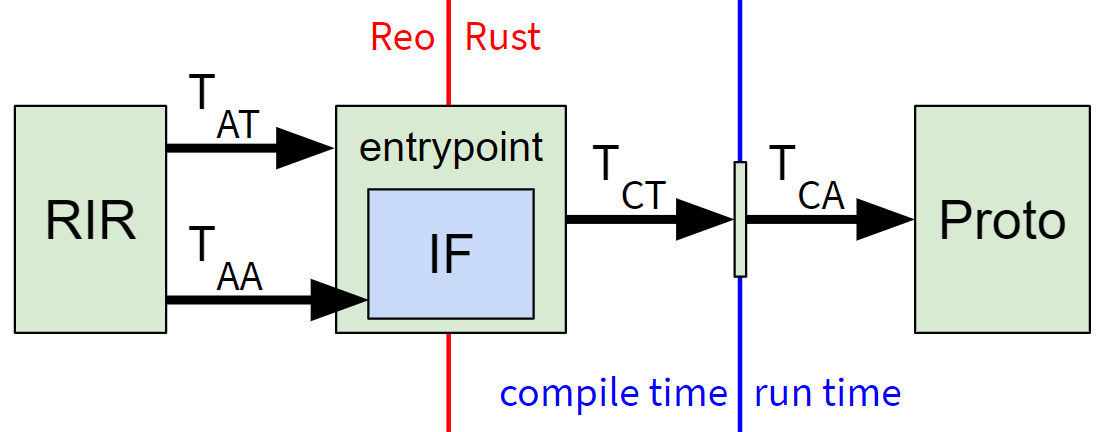
\includegraphics[width=0.80\textwidth]{pipeline.png}
	\caption[TODO.]{The translation pipeline from the Reo compiler's internal representation (`RIR') to executable Rust, expressed in terms of the translation subtasks defined in Section~\ref{sec:sub_tasks}. The majority of the specification is represented in the imperative form (`IF'), which serves as the representation at the boundary between Reo and Rust.}
	\label{fig:pipeline}
\end{figure}

\subsection{Enabling Future Expansion}
Our observation that a significant portion of the Reo compiler's translation work will be shared between backends for different language targets. In our work, we concentrate on the class of languages we consider to be \textit{imperative} in particular. Section~\ref{sec:imperative_form_sec} makes more explicit what characterizes these language targets by defining imperative form. We observe an opportunity to deduplicate this work by promoting this form a new intermediate representation that the Reo compiler may use to facilitate a hierarchal approach to code generation. This vision would generalize the concept of an intermediate representation, making it possible to express and exchange the same Reo protocol formulated such that different tradeoffs between generality and specificity can be made. 

For this work, we relegate imperative form to a tool unique to the generation of the Rust language. The user is not aware that this form exists, as its usage is not user-facing, known only to the Rust backend and the Reo-rs library as a practical representation of Reo protocols. The Reo compiler emits a Rust source file when targeting the Rust language, such that it adheres to the precedent set by the compiler's other backends: Java, for example. For now, our Reo backend emits code in the Rust language. 


%This sentiment is reflected by the existing backend for the Java language in its dependence on a Reo-oriented Java library for defining objects which all Reo-generated code has in common. However, our solution differs from that of the Java version by not emitting Java code in a form in which it can be directly executed. Instead, 
%
%
%
%\hl{
%	code generation is weird. we are doing meta programming. we have multiple languages, multiple compilers. if we have work to do, asking "who and where" becomes a nontrivial question. 
%}
%
%
%The Reo compiler has an existing backend for generating Java code. It works by generating Java according to the structure of a \textit{template generator}. In this manner, it can be thought of as performing all code-generation subtasks at the same time directly from the compiler's intermediate representation. However, the extent to which the Reo compiler is \textit{coupled} to the Java language is reduced through the reliance on a Java library for the granular implementations of structures that are common to all protocol objects; rather than generating these classes each time, the Reo compiler simply generates a dependency. For example, the library defines a \code{Component} interface, for which the code generator produces a protocol-specific implementor class. Consequently, a significant part of the $T_{run}$ subtask (subtasks are defined in Section~\ref{sec:sub_tasks}) is delegated to this library.
%
%For $T_{type}$, help comes from the Reo compiler itself, which in its current form was developed with support for Java in mind. This is visible in its internal representation. For example, types for which no explicit data type annotation was included are assigned the \code{Object} type, which encapsulates all types that may be concretely chosen for transmission through ports. This design essentially uses \code{Object} as a universal type, relegating the task of \textit{type reflection} (determining concretely which `variant' of \code{Object}) to the user themselves. This approach is sufficient in the case of Java, as \code{Object} supports all the behavior relied about by the Reo protocol object at runtime, namely (1) data-equality checks, (2) data movement, and (3) data replication. In the chapter to follow we discuss how this approach introduces safety concerns. In a nutshell, Reo-generated Java erroneously assumes that the replication of \code{Object} references preserves Reo's value-passing semantics, resulting in data races.
%
%Only $T_{seq}$ is performed almost entirely by the template generator. For simple protocols, this task is relatively easy, as there is not much to add when actions are largely concurrent. For example, replicating the contents of a memory cell into a set of others is simply done in Java by first reading an object reference, and then overwriting the others one at a time. However, ordering dependencies must be resolved very carefully in the general case. The current Java code generator is susceptible to erroneously observing value $x$ at memory cell $M$ in the event that the observation is synchronous with $M$'s value being overwritten by $x$. Even with the help of the template generator, this translation is sufficiently complex to make detection of these bugs difficult.
%
%Rust is able to mimic Java's approach to create a similar backend through the explicit use of \textit{dynamic dispatch}, such that types can be collapsed to something analogous to Java's \code{Object} class. If done na\"ively, the resulting backend would inherit the problems of its predecessor, and new ones to boot; the Java-like approach is not idiomatic in the context of Rust; it would not make good use of the extensive control of systems resources unique to a systems language. Chapter~\ref{sec:protocol_runtime} to follow goes into detail about the properties of the protocol runtime. Here, it suffices to say that we wish to implement a runtime that does not restrict port data types to those that are heap-allocated. Furthermore, our runtime wishes to perform more extensive optimizations, relying on the unique abilities of our systems language to manipulate its resources at a low level. All these extensions pose a problem in particular for $T_{run}$, as runtime properties directly influence how the executable protocol objects are represented. Our work in unremarkable in its solution to this problem: we delegate~$T_{seq}$ to a Rust library. However, we make this separation more extreme. In a nutshell, we wish to partition the work of code generation into two clear \textit{phases}, the former of which performs tasks~$T_{seq}$ and~$T_{type}$, and the latter of which performs $T_{seq}$. To minimize coupling between the modules performing these tasks, the interface between phases is made terse, unambiguous and explicit in the definition of a new intermediate representation of protocol connectors: the \textit{imperative form}.
%
%\subsection{Temporary Simplifications}
%\label{sec:temporary_simplifications}
%Our intention is to isolate the Reo backend from Rust's specifics as extensively as possible. In this manner, we decouple the modules responsible for the code-generation subtasks in accordance with good software engineering practices. Furthermore, it facilitates the \textit{reuse} of the first phase of the code generation process for \textit{other} imperative programming language targets. The section to follow defines imperative form to be as target-language agnostic as possible. However, for the sake of minimizing the disturbance to the Reo tooling ecosystem, we still embrace the per-target structure for Reo code generation for now. As such, the Reo compiler still specifies a Rust language target, and emits executable Rust source as a result. Our representation of the \textit{imperative form} is expressed in Rust syntax (as the \code{ProtoDef} type) such that this reliance on an intermediate representation is invisible to the end user. As far as they are concerned, Reo generates native Rust that just happens to \textit{somehow} make minimal use of Rust-specific syntax. \code{ProtoDef} corresponds closely to the definition of imperative form, facilitating this decision being overturned in future with minimal effort.


\section{Imperative Form}
\label{sec:imperative_form_sec}
In this section, we define \textit{imperative form}, a novel intermediate representation for the behavior of Reo protocols, such that they more closely correspond to their final representation in some imperative language. In the protocol translation pipeline, this form is the result of completing translation subtasks $T_{AA}$ and $T_{AT}$, as they are defined in Section~\ref{sec:sub_tasks}.

\subsection{Concept}
The Reo compiler's internal representation does not ergonomically facilitate execution, primarily because it does not define the \textit{order} in which values are accessed, created and moved. Programmers using imperative, sequential languages are very used to thinking in terms of procedures which manipulate the state of variables \textit{in scope} with the order implicit in their control flow. Often, interpreters or compilers provide safety properties by tracking over the execution and emitting errors whenever a variable access is invalid.

Essentially, imperative form makes explicit the ordering between symbolic \textit{actions}; if executed in the specified order, it is guaranteed that (1) variable accesses are always valid, and (2) it is clear at which moment the rule has \textit{fired}.

\subsubsection{Relationship to Reo and Target Languages}
Imperative form represents a protocol whose translation from Reo to an imperative language has been completed as fully as possible, but stopped short of introducing implementation and language specifics. Thus it is still a specification, free from particular syntax, and rendered in terms of \textit{symbolic} identifiers and data types to be resolved in the manner befitting the target language. In terms of the generation subtasks defined in Section~\ref{sec:sub_tasks}, imperative form represents the completion of~$T_{seq}$ and~$T_{type}$, but not~$T_{run}$.

The translation from Reo's internal representation to imperative form is \textit{lossless}, and so any language compiling from the former would also be able to compile from the latter. However, the utility of this representation is the increase in \textit{explicitness}, which results from the ordering of actions. This ordering follow from the fundamental assumption of imperative form: a value can only be accessed \textit{after} it has been created. It also inherits an assumption of the Reo language itself; namely, all values and their identifiers can be assigned a static data type. Imperative form assumes that the target language can assign static data types to ports. However, this assumption is shared by Reo itself, and does not present a problem for untyped languages. For imperative languages without types, ports can simply share some universal~\code{Any} type, satisfying this assumption trivially.

\subsubsection{Rules as Transactions}

The Reo compiler's internal representation partitions the work of a rule into its \textit{guard} and \textit{assignments}. This is already a step in the direction of imperative computation, observing that some work (the guard) must be performed \textit{prior} to deciding whether the rule \textit{fires}, in which case the assignment follows. As the protocol does not define the moments when it will evaluate the guard, it is necessary that this evaluation has no side effects i.e.,\ observable effects to the outside world. In essence, Reo's internal representation formulates a rule as a two-element sequence where the first (the guard) is \textit{transient}, and may end the rule's execution early, and the second (the assignment) exhibits \textit{observable effects}, namely, the results of the rules \textit{firing}.

Imperative form adopts this notion of ordering, but generalizes it to a sequence of arbitrary length. For our purposes, it suffices to continue requiring a single \textit{last} action to represent the assignment. For all prior actions:
\begin{enumerate}
	\item they have a defined means of being \textit{undone}, i.e.,\ the action must be reversible. It follows that each action cannot have any immediately-observable effects,
	\item they may conditionally trigger an \textit{abort} event, which occurs after their evaluation completes.
\end{enumerate}

Effectively, we represent each of the protocol's rules as a \textit{transaction}. All actions but the last represent work \textit{prior} to commitment, reading from data, creating temporary values or triggering an abort. If the last action is reached without aborting, the rule has \textit{fired} and aborts are no longer possible; the final action is then guaranteed to be executed, complete with any of the rule's observable effects. 

\subsubsection{Action Granularity}
Imperative form represents a protocol's defined interaction as actions to be computed in the specified sequence. At this stage, our representation is still symbolic; actions do not necessarily correspond 1-to-1 with concrete operations in the target imperative language, and their representation of actions is unspecified as long as they preserve the properties of imperative form. To avoid underspecification, we represent actions at the coarsest granularity possible to avoid \textit{overspecifying} the ordering of concurrent operations.

The simplest imperative form rules can be represented with a single action; implicitly, the rule has a trivial guard, and consists entirely of some guaranteed \textit{assignment}. For example, a rule with a trivial data constraint may be represented as a single, trivial action; the rule always fires, to no effect.

Connectors become more complex as they rely on the creation of temporary variables. For example, consider a protocol in RBF with data constraint $X=f(X)$ and synchronization constraint $\{X\}$ with only input (putter) port~$P$. This rule can be understood as ``$X$ fires \textit{if} the results of function~$f$ on its put value is equivalent to the value itself''. Here, the result of $f$ clearly cannot be inspected until \textit{after} it is computed. We are able to represent this rule with an action sequence of length three: (1) Create temporary value $f_X$ by executing $f$ given argument $X$. (2) Trigger an abort if $f_X\neq{}X$. (3) The rule has fired; do nothing other discarding values $X$ and $f_X$.


\subsubsection{Valid Value Access}
Imperative languages often prohibit using variables \textit{prior} to definition. Usually, the only case in which a variables access becomes invalid if it goes out of scope. Rust and affine languages generalize this notion, working to keep track of the moment when a value is \textit{consumed}, after which its access is invalid. 

For our purposes, it is useful to allow values to \textit{become invalid}. In the context of imperative form, this allows any actions to \textit{empty} memory cells, as long as they still follow the rule (i.e.,\ they are able to \textit{undo} the emptying). The motivation behind this extension is Reo's ability to express the access of the value of a memory cell both before and after it is overwritten. We are able to represent these kinds of interactions with sequential actions if we are able to \textit{empty} a filled memory cell's contents elsewhere. 

Ultimately, we elaborate our notion of value validity to correspond more closely with the actions an affine-typed compiler would perform: in reading over actions from top to bottom, \textit{inaccessible} identifiers become \textit{accessible} when their values are created, and accessible identifiers become inaccessible if their values are explicitly emptied. A variable access is valid only if it was accessible at the end of the previous action. This formulation makes clear the need of some means of deciding which values are \textit{initially accessible}. Our solution is made apparent in the definition of IF to follow.

\subsection{Definition}
\label{sec:imperative_form_definition}
Here we define \textit{imperative form} (`IF') concretely, and explain how its definition corresponds with the intuition behind it. Firstly, an IF contains a structure which corresponds to a \textit{symbol table}; this does the work of assigning symbolic \textit{data types} to ports and memory cells. Ports must also be annotated with an explicit \textit{orientation} (i.e.,\ input or output). Other symbols are also represented here, for example, the names and the argument types for any named functions.

More interesting are the \textit{imperative rules} listed for an IF. Each rule is given by $(P,I,M)$ where:
\begin{enumerate}
	\item \textbf{Premise $P$}\\
	A tuple of three \textit{identifier} sets $(P_R, P_F, P_E)$. $P_R$~is the \textit{synchronization constraint}, i.e.,\ the set of ports identifiers whose values must be `ready'. $P_F$ and $P_E$ are the sets of \textit{memory variables} which must be known to be full and empty respectively, such that it is known whether they can be read or written from. The rule can certainly not consider firing unless all ports are ready and all memory cells are in the specified states.
	
	\item \textbf{Instructions $I$}\\
	A list of reversible \textit{instructions} which are performed in sequence. These instructions have no immediately observable effects, such that they can be reverted in the event of an \textit{abort}. Concretely, each instruction is one of:
	\begin{itemize}
		\item $check(p)$\\
		Trigger an \textit{abort} if predicate $p$ over data is satisfied.
		\item $fill_P(m, p)$\\Fill an empty memory variable $m$ with the result of a predicate $p$ over available data. The value's data type is implicitly \textit{boolean}.
		\item $fill_F(m, f, a)$\\
		Fill an empty memory variable $m$ with the result of invoking function $f$ with parameters $a$, a list of references to data variables with length matching the arity of $f$. It is incorrect for $f$ to \textit{mutate} its arguments, as this would result in observable effects which cannot be rolled back.
		\item $swap(m_0,m_1)$\\
		Swap the values in two memory variables~$m_0$ and~$m_1$.
	\end{itemize}
	If an abort is triggered by $check$, any swapped memory cells are swapped back, and any memory cells whose values were created by $fill_P$ or $fill_F$ are destroyed.
	
	\item \textbf{Movements $M$}\\
	A mapping from identifiers of \textit{values} to the identifiers of getter ports and empty memory cells. This represents the final action of an imperative rule executed if and only if the rule \textit{fires}.
\end{enumerate}

Our definition represents an elaboration of the underlying concept. $P$ and $I$ contain only \textit{transient} actions, which have no immediately-observable effects, and are able to handle the rule aborting such that their actions are \textit{undone}. $P$~is distinguished as it serves a dual purpose: (1) it establishes which values are initially \textit{accessible}, and (2) it tersely expresses an immediate conditional abort in the event the ports and memory cells are not in the states defined. $M$~is the final action, performed if and only if the rule commits. It defines what happens to all of the \textit{accessible} values still `in scope' at the end of the rule's execution. $I$~contains everything else, representing an arbitrary sequence of transient computation. These actions are subject to handling the rule being aborted, and thus our definition includes only reversible actions. Data is prohibited from being irrecoverably lost during $I$ actions, as otherwise the actions could not be \textit{undone} in the event of the rule aborting. This has three notable consequences:
\begin{enumerate}
	\item $fill_F$ can only rely on \textit{pure} functions, i.e.,\ their execution in and of itself must not be observable to the outside world.
	\item $fill_F$ and $fill_P$ can only write to \textit{inaccessible} values, i.e.,\ they cannot overwrite accessible values.
	\item Accesses of any values must not mutate or consume the original, e.g.,\ using a value as an argument in $fill_F$.
\end{enumerate}

Conceptually, the final, committing action of the rule is able to perform any computation at all (provided it does not break any data-access rules) safe in the knowledge that its actions are allowed to be \textit{irreversible}. However, our definition constrains what $M$ can express significantly. $M$~only defines the fate of the \textit{accessible} values that remain after all other actions are performed. Essentially, $M$ maps each value to the set of locations to which it is moved. This representation makes it trivial to distinguish the cases where values are discarded (0 destinations), moved linearly (1 destination) or replicated (multiple destinations). This design is convenient for languages that require their values to be more explicitly managed. For example, languages with \textit{affine types} (e.g.,\ Rust) must simulate the replication of values by creating new affine resources from the original, and managing the replicas explicitly.  \textit{Relevant} data types (which must be used \textit{at least once}~\cite{walker2005substructural}) must handle empty destination sets by either emitting errors, or simulating destruction.\footnote{A relevant language may simulate the destruction of a value by moving it to some \code{Destroyed} destination with special semantics.} There are many other reasons a language may want to specialize the way its values are used. For example, an implementation in C++ may need to inject \code{free} calls to avoid leaking memory in cases where pointer-values are discarded.

As an example to demonstrate intermediate representation, the RBA rule in the previous section with data constraint $X=f(X)$
and synchronization constraint $\{X\}$ can be represented in the imperative rule with:

\vspace{1em}
\noindent{}
\begin{tabular}{r|l}
	\centering
	&  value \\ \hline
	premise	&  $(\{X\}, \enskip\{\}, \enskip\{f_X\})$ \\
	instructions	& $[fill_F(f_X, f, [X]), \enskip{} check(X = f_X)]$ \\
	movements	& $\{X \rightarrow{}\emptyset{}, \enskip f_X \rightarrow{}\emptyset{}\}$ 
\end{tabular}
\vspace{1em}

\section{Translation Pipeline}
\label{sec:translation_pipeline}
This section details the implementation of the translation pipeline from the Reo compiler's internal representation (`RIR') of Reo protocols to executable Rust. The section is structured to describe the translation process as a sequence of sequential stages. Unbeknownst to the user, the pipeline extends well after the Reo compiler has emitted Rust code. Subsections are titled according to \textit{when} the translation takes place.
%In this section be describe how Reo's internal representation (`IR') of protocol specifications is translated to a Rust protocol object. As per the design in Section~\ref{sec:two_phase}, this process involves generation steps partitioned over two distinct phases with imperative form (`IF') in between. Here, we describe this process beginning to end. Throughout this section, we refer to the generation process in terms of its three distinct subtasks $\{T_{seq}, T_{type}, T_{run}\}$, defined in Section~\ref{sec:sub_tasks}.


\subsection{At Reo Compile-time}
\label{sec:translation_phase_1}
The Reo compiler is extended with a backend for translating RIR to a Rust source file. This translation stage is concerned with performing $T_{A,A}$ and $T_{A,T}$, and representing them as a single rust \textit{entrypoint} function in the emitted Rust source. The user is able to import this source as a dependency into their own project, whereby the entrypoint serves as a means for their program to construct the Rust object which implements the appropriate Reo protocol specification, as described in~\ref{sec:reo_motivation}.

\subsubsection{Action Sequencing}
$T_{A,A}$ necessitates transforming a each of the protocol's rules into a sequence of symbolic actions. The most significant work occurs as a result of how differently \textit{values} are represented. IR is declarative, representing the result of a rule's firing as an \textit{assignment}, mapping \textit{destinations} (getter ports and empty memory cells) to \textit{terms}. IR already represents a significant transformation from RBF in isolating these values on a per-destination basis. 

To begin, we describe the na\"ive approach to translate IR to IF a rule at a time.

Our translation procedure initializes all three fields $\{P, I, M\}$ of an imperative rule as initially empty, and populates them incrementally by recursively traversing the IR rule's assignments. Each such assignment is ultimately represented in~$M$, where \textit{terms} are rather represented by identifiers. For some terms the mapping to identifier is trivial. For example, the value put by a port can use the identifier of the port itself. For others, it may be necessary to introduce \textit{fresh} identifiers, representing \textit{temporary variables} to be created. In either case, the \textit{term} is traversed recursively to (1) collect these identifiers, and to (2) populate the premise~$P$ such that the rule is fired given access to all of the relevant memory cells and ports.

$I$ is populated last by three kinds of actions. Firstly, the exceptional cases for which memory variable~$q$ will be both read and written to are treated. If necessary, a fresh temporary variable is introduced by appending an instruction $swap(q, q_{temp})$ where $q_{temp}$ is some fresh variable; $q$'s previous and next values may be read and written unambiguously, distinguished by identifiers $q_{temp}$ and $q$ respectively. Second, $I$ is appended with $fill_P$ or $fill_F$ instructions to create every other temporary variable in a manner befitting the \textit{term} that represented them in the IR's assignments, i.e.,\ the result of invoking a function with port values as arguments. Finally, $I$~ends with a single $check$ to evaluate the rule's guard, initiating an abort if it is evaluates to \textit{false}.

As it was described thus far, our procedure is able to correctly render any IR rule in IF with the necessary properties. For the sake of minimization or performance at runtime, at least three optimization opportunities may elaborate on this procedure, producing semantically-equivalent results.

\begin{enumerate}
	\item Terms that occur repeatedly within assignments throughout the same IR rule may have their \textbf{values deduplicated} by assigning them all the same \textit{identifier}. Care must be taken to ensure that the instruction to create its value is inserted only once, sufficiently early that its creation precedes its \textit{earliest} access. Note that each original occurrence still corresponds with a \textit{destination} in the resultant~$M$ mapping. To clarify, consider the example with getter ports~$A$ and~$B$ both assigned terms corresponding to $f(C)$ where $f$ is some function and $C$ is a putter port. Here, one temporary variable $f_C$ to store the result of $f(C)$ is sufficient; it is simply moved to two distinct destinations, reflected in the mapping $f_C\rightarrow\{A,B\}$ in~$M$.
	
	\item The large, monolithic \textit{check} instruction that acts as a guard to the rules firing can be fragmented into \textbf{numerous guard instructions}. The utility of this is the ability to rearrange their ordering. For best results, it is beneficial to move checks as early as possible, such that less work is performed prior and subsequently to an abort whenever the check \textit{fails} at runtime. To be correct, care must be taken not to move guards so early such they precede the creation of any temporary variables their evaluation accesses. For example, consider an IR 
	whose guard is $A\wedge{}B$, where~$A$ and~$B$ are subformulas that reason about subterms whose evaluation necessitates the creation of temporary values~$t_A$ and~$t_B$. By fragmenting $check(A\wedge{}B)$ into $check(A)$ and $check(B)$, we are able to move the former such that it follows the creation of $A$, but not of $B$. Effectively, the rule is able to \textit{short circuit} its evaluation at runtime, circumstantially avoiding the creation and destruction of the temporary value identified by~$t_B$.
	
	\item \textbf{Static analysis} of values may conclude that a \textit{check} instruction is a tautology, making it safe to omit. Similarly, the presence of even one contradictory \textit{check} makes it possible to discard the rule entirely. This optimization is particularly useful in combination with optimization (2).
\end{enumerate}

\subsubsection{Type Classification and Constraining}
Our backend performs task $T_{A,T}$ to generate the IF such that the identifier of every port, memory cell, and temporary variable is assigned a symbolic type annotation, such that:
\begin{enumerate}
	\item the types of identifiers match if they exchange values or are checked for equivalence.
	\item data types are boolean if they occur in a context in which only boolean types are permitted, i.e.,\ as the predicate of a formula.
	\item the type defines all the operations in which it may be involved at runtime. This includes operations for \textit{replication}, checking \textit{equality} of values and so on.
\end{enumerate}

Our backend performs this work in tandem with the work of $T_{A,T}$ described in the previous section. Initially, every identifier is assigned s fresh symbolic type with no constraints, representing a data type unrelated to any other, and having no need of any defined operations. In traversing the IR rules, \textit{constraints} are collected, associating them to the relevant identifiers. Incrementally, \textit{type constraints} are collected, accumulating requirements for the properties of types. For example, the type associated with a value is checked for equality, irrevocably acquiring the \code{eq} constraint, marking the need for it to define an operation to check value equality. In some cases, a relationship between identifiers causes their types to be \textit{unified}. For example, a data movement from putter~$P$ to getter~$G$ unifies their types, resulting a new type with the union of their constraints. If the requirements on types are \textit{contradictory}, an error is emitted by the Reo compiler. For example, it is an error to provide types $A$ and $B$ with different explicit data type annotations, yet have them exchange data.

Ultimately, the constructed IF associates a symbolic type with every mapping in its symbol table.

\subsubsection{Rust Formatting}
Once all the data has been prepared, the Reo compiler emits its contents formatted according to Rust's syntax. Listing~\ref{listing:generated} gives an example of the result: a single \code{instantiate} function reflecting the cumulation of the work of this phase. Observe that in this example, a single symbolic data type \code{T} was identified. As expected, the majority of the information is contained in the \code{ProtoDef} type (beginning on line~5), which is nothing more than a Rust-formatted rendering of the protocol's imperative form behavior specification. The sections to follow explain what happens next.

\begin{listing}[ht]
	\centering
	\inputminted[]{rust}{generated.rs}
	\caption[TODO.]{The Reo-generated Rust source given the $fifo1$ connector's Reo specification as input. Section~\ref{sec:translation_pipeline} explains how this representation bridges the gap between the Reo and Rust languages. The \code{ProtoDef} type on line~5 specifies the protocol's behavior in imperative form, as it appears embedded into Rust's syntax.}
	\label{listing:generated}
\end{listing}

\subsection{At Rust Compile-time}
A Rust programmer makes use of the generated Rust code by importing it into their own program as a library. To interface with its contents, they are required to import Reo-rs as well. Section~\ref{sec:user_facing} explains the API this library presents to users for acting on these protocol objects from their own code. 

As the name suggests, the \textit{instantiate} function serves as the user's \textit{entrypoint} for instantiating protocol objects. This function is invoked from their own Rust code in the usual way. Section~\ref{sec:rust_language} explains how Rust relies on dispatch for generic type resolution. Previously, Section~\ref{sec:translation_phase_1} explained that the output of the Reo compiler is a Rust source file containing a single entrypoint function. Rather than implementing it ourselves, our solution is for the definition of this function to effectively delegate subtask $T_{C,T}$ to the Rust compiler itself. From the user's perspective, the entrypoint is a function like any other; at the call-site within their own programs, they are able to specify concrete choices for the generic types themselves.
This approach has three benefits: (1) We make use of an existing resource, which is not only easier, but is also good practice as it avoids the fragility that would otherwise follow from redundancy, (2) the result is idiomatic for the Rust language, and ergonomic for users to use in conjunction with other generics in their own programs, and (3) once Reo has emitted the entrypoint, a Rust programmer is able to use it to construct protocol instances for any choice of concrete types.

Using the Rust compiler in this way is achieved by the Reo compiler crafting the entrypoint such that its generic type arguments are annotated with the appropriate Rust trait bounds. In effect, we communicate to the Rust compiler the operations which the user's code chosen types must support. This makes for a pleasant user experience, as their uses of the entrypoint will be checked for correctness by the Rust compiler as is the case for any other aspect of their program.

%\subsubsection{Delegated to the Rust Compiler}
%Section~\ref{sec:temporary_simplifications} explains that our current implementation of the Rust backend for the Reo compiler makes the temporary simplification of emitting Rust source code directly. This approach adheres with the Reo compiler's idiom of code generation per target language, but also it simplifies our work overall as we are able to effectively \textit{delegate} some of the translation work to the Rust compiler itself. Both of these simplifications are inspired by Reo's Java code generator, whose direct-to-Java code generator delegates these tasks to the Java compiler in the same manner:
%\begin{enumerate}
%	\item \textbf{Parsing}\\
%	Per our design, IF should be emitted in a format agnostic to the imperative language target; good contenders are common data serialization formats such as JSON or YAML. Ultimately, IF is translated to the syntax understood by the target language such that it can be integrated into the user's programs. While Rust is the only language target, we are able to unify these steps by emitting Rust syntax as a usable dependency directly.
%	
%	\item \textbf{Type Resolution}\\
%	Our symbolic data types are exposed as \textit{generic types} in the emitted source; effectively, the user's Rust compiler makes concrete these symbolic types at the call site, as is idiomatic in the Rust language.
%\end{enumerate}
%
%The second task is most interesting, as care must be taken to represent our generic types in a manner that the Rust compiler will accept. Previously, we described how requirements on our symbolic types are discovered throughout $T_{type}$. Here, these constraints are communicated to the Rust compiler in the generated syntax. This delegates the task of enforcing these constraints to the user's Rust compiler. Listing~\ref{listing:generic_resolve} gives an example of a signature for a Reo-generated Rust function with constrained generic types~\code{X} and~\code{Y}. Observe that the majority of the functions contents are the definition of a~\code{ProtoDef} type, which is the Rust-embedding of our IF. 
%
%\begin{listing}[ht]
%	\centering
%	\inputminted[]{rust}{generic_resolve.rs}
%	\caption[Simple Reo compiler Rust output.]{Example of a Reo-generated Rust output for a simple connector which replicates values of port $P$ to ports $\{C0, C1\}$. The user is able to construct \code{ProtoHandle}, a handle to an executable protocol object by invoking function~\code{build\_protocol\_1}. The caller determines the concrete choice of the generic type~\code{T}, but the Rust compiler will enforce that this choice is constrained such that it implements~\code{Clone} (the type's values can be replicated). The contents of the function consist predominantly of the construction of an instance of \code{ProtoDef}. In combination with \code{MemInitial}, these types represent the Rust-embedding of the protocol's imperative form specification.}
%	\label{listing:generic_resolve}
%\end{listing}

\subsection{At Application Runtime}
\label{sec:translation_phase_2}

The user's program has been compiled by the Rust compiler, the resulting binary can be directly executed. Represented somewhere within is code which implements the Reo-generated \code{instantiate} function. This function constructs and returns an instance of \code{Proto}, indirected behind a \code{ProtoHandle}. These types and how they work to implement their associated Reo protocol at runtime is explained in Section~\ref{sec:protocol_objects}. Here, it suffices to say that Reo-rs relies on the Reo-generated \code{instantiate} function to construct a \code{Proto} such that its contents facilitate the intended behavior, including specializing it to implement the associated Reo protocol in particular.

At runtime, the user's program is evaluated in the usual way. The final subtask of protocol translation, $T_{CA}$, occurs only at the moment \code{instantiate} is invoked. Owing to Rust's imperative nature, what happens next occurs a sequence of four distinct steps, corresponding with the initialization of the four variables in the scope of \code{instantiate}, as they appear in the Listing~\ref{listing:generated}. Throughout this section we refer this listing to exemplify the translation steps.

\subsubsection{Type Erasure: \code{type\_info}}
To make it possible to represent any and all protocol objects with the single \code{Proto} type, it is necessary to \textit{erase} the types of port values, representing them instead as data such that their behavior may be later recovered through \textit{reflection}. The first step of \code{instantiate} is to perform this erasure. Its counterpart is explained in Section~\ref{sec:type_reflection} in the following Chapter. As can be seen in the example, this step is trivially represented by the Reo compiler, relying on the definition of \code{TypeInfo} in Reo-rs.

\subsubsection{Memory Initialization: \code{mem\_init}}



In the original textual Reo specification, the initial values of a protocol's memory cells is defined by strings (as a result of the format). To afford the user's choice of arbitrary types, we require that the original text can be translated into a value of the correct type to initialize the protocol's memory cells. Rust defines the \code{FromStr} trait characterize types which have the property that their instances can be constructed by parsing a string at runtime. The entrypoint function is safely able to rely on the corresponding \code{from\_str} operation to be defined for the type, as care was taken to include it as a type constraint. The result is a \code{MemInitial} instance, storing instances of initialized values precisely as specified.

\subsubsection{Imperative Specification: \code{proto\_def}}
As explained previously, the Reo backend embed the imperative form specification in Rust's syntax such that the result is a dependency which the Rust compiler can understand. At runtime, this step necessitates that a \code{ProtoDef} instance be built, only to be read on the next line and subsequently discarded. Conceptually, this step could be performed at compiler-time by defining the \code{ProtoDef} in terms of types that the Rust compiler is able to embed into the text section of the generated binary. This would avoid the work of constructing the \code{ProtoDef} with every instance, as (to follow) we see that one \code{ProtoDef} is able to instantiate any number of \code{Proto} instances. This construction is represented inlined here to facilitate future expansions to Reo-rs in future, allowing protocols objects to be manipulated at runtime. Reformulating \code{ProtoDef} would inhibit these efforts. As \code{instantiate} is not a performance-sensitive function, investigating workarounds for this overhead was not a priority in this project.

\subsubsection{Construction: \code{built\_proto}}
The combination of \code{ProtoDef} and \code{MemInitial} represent (a specification of) the behavior, and initial state of an executable protocol object respectively. The final step is to put it all together and perform the only remaining subtask:~$T_{C,A}$. Reo-rs encapsulates this work in the \code{build} method defined for the \code{ProtoDef} type, visible in Listing~\ref{listing:generated} on line~32. 

Completing subtask $T_{C,A}$ in this context consists of (1) initializing a protocol object complete with auxiliary bookkeeping structures, and (2) translating the imperative form behavioral specification into something conducive to execution. \code{Proto} structures are instantiated complete with various fields to facilitate the granular operations that are defined by Reo-rs. Structures are added which have no clear parallel in the imperative form specification, but whose precedence is nevertheless essential at runtime: for example, semaphores and control message channels. Imperative form rules are significantly preprocessed before being included in \code{Proto}. This performs two vital functions:

\begin{enumerate}
	\item \textbf{Optimizes Representation for Execution}\\
	\code{Proto} represents the ultimate departure from the initial Reo specification. in Chapter~\ref{sec:protocol_runtime} to follow, we explain how the contents of \code{Proto} are accessed directly while in use as a communication medium at runtime. As such, the representations of \code{ProtoDef} and \code{Proto} are not the same. Where \code{ProtoDef} prioritizes terseness and readability in the use of symbolic port and function names, the translation to \code{Proto} resolves them to concrete data structures for cheaper access. For example, indexes into a vector replace symbolic port names.
	
	\item \textbf{Ensures Internal Consistency}\\
	In this scope of this project, we are safe in our presumption that the Reo compiler can be trusted to create only internally consistent \code{ProtoDef} structures. However, the code generation process crosses a boundary between two compilers, and is designed to minimize their coupling by condensing the data that passes between them. As a good practice, Reo-rs will check that the \code{ProtoDef} describes \textit{some} valid, sensible protocol. Owing to its increased explicitness, imperative form exposes a larger `surface area' for the introduction of inconsistencies, accidental or otherwise. To make error handling ergonomic for the user, \code{build} returns an informative error structure with information about the inconsistency. Listing~\ref{label}	shows the resulting type signature of \code{build}, including some examples of possible error variants.
\end{enumerate}


\begin{listing}[ht]
	\centering
	\inputminted[]{rust}{build.rs}
	\caption[TODO.]{Signature of the~\code{build} function. Its inputs are (1) an immutable reference to a \code{ProtoDef}, which is used to determine the protocol's behavior, and (2) a \code{MemInitial}, which stores initialized memory cells to be incorporated into the protocol's state. The return result is an enumeration type, returning \code{ProtoHandle} upon success, and a tuple on failure, whose elements are, respectively (1) the index of the imperative rule where the error occurred if applicable, and (2) another sum type, communicating the nature of the error with additional information. }
	\label{listing:build}
\end{listing}

Listing~\ref{listing:generated} demonstrates how the result of \code{build} is returns the resulting protocol object directly. Observe that Listing~\ref{listing:build} shows the protocol object returned indirectly, via a \code{ProtoHandle}. The relationship between these objects and the definition of their behavior at runtime is detailed in Chapter~\ref{sec:protocol_runtime} to follow.
%
%
%Subtask $T\_{CA}$ represents the translation of the protocol's abstract (but imperative) behavior to a form executable in Rust. To minimize the work of the Reo compiler itself, and to avoid duplication in the user's programs, this work is extracted to Reo's supporting Rust library, Reo-rs. Within, the \code{build} function instantiates a new \code{Proto} object. This function is parameterized with a \code{MemInitial} (which is consumes), and a \code{ProtoDef} (which it reads). The majority of the entrypoint function's body concerns itself with the construction of the \code{ProtoDef}, which is nothing more than the Reo-generated imperative form embedded in Rust's syntax. 
%
%During \code{build}, Reo-rs works to preprocess its inputs
%
%\subsubsection{Internal Consistency Check}
%
%Our work follows the precedent set by the Java code generator in relying on a library in the target language to define the lion's share of the behavior for our runtime protocol objects. For Rust, these definitions are bundled into the \textbf{Reo-rs} library, which is added as a dependency to the code generated by the Reo compiler's backend. Chapter~\ref{sec:protocol_runtime} explores the architecture and behavior of our executable protocol objects in detail. For now, it suffices to say that our approach is to represent executable protocols as extensively preprocessed \textit{data structures} which then drive the behavior of a lightweight \textit{interpreter} at runtime. This data representation is often called \textit{commandification}~\cite{nystrom2014game}. 
%
%
%\subsubsection{Protocol Initialization}
%Listing~\ref{listing:generic_resolve} gives an example of Reo-generated Rust source. Previously, we explain how this representation delegates some of the work of $T_{run}$ to the Rust compiler itself. The remainder of $T_{run}$ is defined in the \code{build} procedure (visible is the listing on line~23) such that this work is performed at runtime whenever a protocol is \textit{instantiated}. As can be seen in the \textit{return value} of the function in the listing, the end result is the construction of \code{ProtoHandle}, a handle to an \textit{executable} protocol object, whose properties are explored in Chapter~\ref{sec:protocol_runtime}.
%
%At this level, the specification used to \code{build} the \code{Proto} is split into two distinct types: \code{ProtoDef} and \code{MemInitial}. The former describes its \textit{behavior}, corresponding most closely with the conceptual design of IF. The latter isolates a simple structure which contains preallocated values for the finished \textit{protocol object}; in effect, it provides the initial values of memory cells. These structures are distinguished for only one reason: \code{ProtoDef} contains no \textit{values}, such that it can be accessed by \code{build} in a read-only fashion. Although it is not taken advantage of by the Reo-generated program, one is able to define a protocol's behavior \textit{once} to be used for the construction of any number of \code{Proto} instances.
%
%\code{Proto} represents the ultimate departure from its original, declarative protocol specification whose purpose is to facilitate execution. Its creation from \code{(ProtoDef, MemInitial)} involves the last remaining subtasks of $T_{run}$:
%\begin{enumerate}
%	\item \code{Proto} is constructed along with data structures necessary for basic operations at runtime. This includes semaphores, channels for \textit{control messages} and so on. This minutia is detailed in Section~\ref{sec:protocol_object_architecture}.
%	
%	\item In construction, the behavioral specification (i.e.,\ imperative form rules) are \textit{preprocessing}  to a form more conducive to efficient execution. For example, symbolic names are replaced with indices, pointers and keys into concrete data structures. The \textit{soundness checks} in the section to follow can be considered preprocessing also, as they ensure a \code{Proto} is constructed such that it is internally consistent, ensuring various runtime properties are invariant and need not be checked at runtime.
%\end{enumerate}
%
%
%\subsubsection{Soundness Check}
%Our backend is novel in that the work of constructing the executable protocol object requires crossing an API boundary. Rather than trusting the well-formedness of the Reo-generated \code{ProtoDef}, Reo-rs will check that its input is internally consistent. By adding these checks, the dependency between the Reo compiler and Reo-rs is \textit{unidirectional}; users are free to safely construct protocol objects using Reo-rs in their applications directly. The most obvious advantage to this approach is an additional layer of safety, allowing for the compiler and Reo-rs to be maintained separately, e.g.,\ if the compiler acquires a bug from a new update, the error cannot propagate into Reo-rs unnoticed. Another advantage is the avenues for future work this opens up. Our approach treats protocol structures as data, facilitating their mutation at runtime, resulting in \textit{dynamic protocol reconfiguration}, although exploring this further is beyond the scope of this work.
%
%In native Rust, the usual variable scoping rules apply to ensure that a symbolic identifier is resolved to a meaningful memory position. These systems are so familiar to us that we usually take the complexity of their work for granted. Rules that are second nature to us require explicit enforcement to replicate the work of the checker. As \code{ProtoDef} \textit{commandifies} the behavior to be later executed, the Rust compiler does not interpret these actions in the normal way, and we must mimic its behavior manually. We take this idea a step further by relying on the \code{ProtoDef}'s \textit{premise} to facilitate a mechanism that mimics the Rust \textit{borrow checker} system; rules trace which variables are \textit{valid} (i.e.,\ initialized) throughout the rule's execution top to bottom, tracking changes as a result of actions filling or swapping their values. In this manner, we are able to catch invalid memory accesses during \code{build}, rather than encountering them at runtime. An additional perk of mimicking this system is our ability to detect the occurrence of values which \textit{must} be consumed during the rule's firing, but whose consumption is not included in the specification. For example, an \textit{imperative rule} may include some putter port $P$ in its ready set (and thus, its synchronization constraint), but associate no \textit{movement} with $P$'s value. A na\"ive implementation which overlooks such occurrences may introduce \textit{memory leaks} for such cases if it takes the specification at face value. Instead, our custom borrow checker will reach the end of of the specified actions and conclude that as $P$ was not explicitly emptied, it will insert a trivial movement $P\mapsto{} \{\}$ to ensure the value is consumed. This is analogous to how Rust's borrow checker inserts \code{drop} calls to destroy local variables which go out of scope unconsumed. By performing this extensive checking, Reo-rs affords an expressive \code{build} function, capable of giving detailed error information in response to an invalid input. The signature of this function is given in Listing~\ref{listing:build}.
%
%
%\begin{listing}[ht]
%	\centering
%	\inputminted[]{rust}{build.rs}
%	\caption[TODO.]{Signature of the~\code{build} function. Its inputs are (1) an immutable reference to a \code{ProtoDef}, which is used to determine the protocol's behavior, and (2) a \code{MemInitial}, which stores initialized memory cells to be incorporated into the protocol's state. The return result is an enumeration type, returning \code{ProtoHandle} upon success, and a tuple on failure, whose elements are, respectively (1) the index of the imperative rule where the error occurred if applicable, and (2) another sum type, communicating the nature of the error with additional information. }
%	\label{listing:build}
%\end{listing}
%
%By restricting our API such that all executable protocol objects are \textit{only} created by \code{build}, our runtime interpreter is able to rely on the properties we guarantee and avoid checking them itself. In this way, checking for soundness is also an optimization.

